% arXiv: force the pdflatex path. Figures are inline TikZ, there are no
% .eps files, and this must stay within the first few lines to take effect.
\pdfoutput=1

\documentclass[11pt]{article}

\usepackage[margin=1in]{geometry}
\usepackage{amsmath,amssymb,amsthm}
\usepackage{mathptmx}
\usepackage[numbers,sort&compress]{natbib}
\usepackage{booktabs}
\usepackage{graphicx}
\usepackage{xcolor}
\usepackage{tikz}
\usetikzlibrary{arrows.meta,positioning,fit,calc}
\usepackage{algorithm}
\usepackage{algpseudocode}
\usepackage{caption}
\usepackage{enumitem}
\usepackage{longtable}
\usepackage[colorlinks=true,linkcolor=blue!60!black,citecolor=blue!60!black,urlcolor=blue!60!black]{hyperref}
\usepackage{fancyhdr}

\pagestyle{fancy}
\fancyhf{}
\fancyhead[L]{\small Functional Self-Awareness for SARSI Agents --- Unified Edition}
\fancyhead[R]{\small Preprint}
\fancyfoot[C]{\thepage}
\renewcommand{\headrulewidth}{0.3pt}

\newcommand{\op}[1]{\operatorname{#1}}

\usepackage{framed}
\definecolor{shadecolor}{gray}{0.93}
\newenvironment{claimbox}[1]{%
  \begin{shaded}\noindent\textbf{#1}\par\smallskip}{%
  \end{shaded}}

\newtheorem{definition}{Definition}
\newtheorem{proposition}{Proposition}

\title{\LARGE Functional Self-Awareness for SARSI Agents\\[4pt]
\Large A Brain-Inspired Dynamic State Space, Unified with\\
\Large Loop-Closure Levels and Deployed Applications}

\author{Chengshuai Yang\\
NextGen PlatformAI C Corp.\\
\texttt{spiritai@platformai.org}}

\date{July 29, 2026}

\begin{document}

\maketitle
\thispagestyle{empty}

\begin{abstract}
\noindent
The SARSI research program now spans two things that have been developed apart: a \emph{brain-inspired dynamic state space} describing what an individual agent knows about itself, and \emph{SARSI-L}, which holds that recursive self-improvement is substrate-indexed and describes how it closes loops across substrate domains from software to stellar engineering. Between them sit four applied systems --- a governed session guider, a scientific discovery agent, a computational-imaging agent, and a deployed multi-agent console --- each carrying its own self-model notation. The result is a corpus that contradicts itself in five specific places: the number of self-model dimensions (nine, ten, twelve, and thirteen appear across documents), the depth of the evidence-authority ladder (five levels in one paper, seven in another and in the shipped code), whether self-awareness is a prerequisite for loop closure (asserted in one document, rejected as circular in another), whether autonomous deployment of a self-modification is permitted (required for Loop~I closure, forbidden by the safety invariants), and whether autonomous goal revision is a milestone or a violation. This paper is the unified edition. It keeps the brain-inspired architecture as canonical --- a ten-coordinate evidence-grounded self-state, specialized asynchronous processors, a bounded global workspace, a predictive self-model corrected by residuals, dual-timescale improvement --- and resolves each contradiction rather than restating it. The central construction is a \emph{two-scale} account: the agent-scale self-state $s_t$ and the system-scale loop-completion profile $\ell_t$ are the same kind of object, both formerly ladders, both replaced by profiles for the same reason, and measured on one shared five-band scale. We define \emph{governed loop closure}, which separates capability closure from authority closure and shows that SARSI-L's Loop~I criterion and the no-self-promotion invariant are compatible once the promoter is defined as a role rather than as a species. Stated in SARSI-L's own machinery, authority closure is exactly the removal of the deploy step from the externally-gated set of its Amdahl bound: until it is granted, that bound caps the software loop's iteration rate at the reciprocal of deploy-authorization latency no matter how capable the agent becomes. This identifies the self-state as an instrument acting on a removable throughput floor rather than on any physical one, supplies the representation of institutions that SARSI-L's final open problem reports missing, and makes the deployed console's authorization timings one of the two measurements that decide SARSI-L's central crux. We unify the corpus's two autonomy vocabularies --- capability ceilings $A_0$--$A_4$ and scientific risk tiers $R_0$--$R_5$ --- into a single admissible-action filter, give a crosswalk mapping every published self-model onto the ten canonical coordinates, and report what the deployed console actually measures today against the framework it claims to implement. The framework remains strictly functional: it defines and measures a control capability and makes no claim about consciousness.
\end{abstract}

\vspace{4pt}
\noindent\textbf{Keywords:} SARSI; functional self-awareness; brain-inspired AI; metacognition; predictive processing; global workspace; dynamic state space; recursive self-improvement; loop closure; intelligence levels; AI governance.

\section{Introduction}
\label{sec:intro}

\subsection{Two literatures, one program}
Two lines of work now describe the same system from opposite ends.

At the \emph{agent} scale, the brain-inspired formulation \citep{yang2026brain} asks what a single autonomous agent knows about itself. It rejects a linear self-awareness ladder in favour of a ten-coordinate state vector spanning identity, situated task state, goals and scope, epistemic status, capability, memory, development, recursive-improvement status, organizational relations, and resource integrity. Specialized processors update those coordinates asynchronously from admissible evidence; a bounded workspace broadcasts what the current decision needs; a predictive self-model forecasts outcomes and is corrected by residuals; a metacognitive controller chooses among acting, tool use, delegation, clarification, abstention, and escalation; and structural self-modification is separated from ordinary state estimation by an evaluation-and-signature gate.

At the \emph{system} scale, SARSI-L \citep{yang2026sarsil} asks how far recursive self-improvement has propagated across substrate domains. Its v3.0 edition makes the governing claim explicit: recursive self-improvement is \emph{substrate-indexed}, an improvement loop is always a loop over some substrate the system can modify, and the binding constraint migrates between substrates. It replaced binary open/closed status with a five-band completion estimate, invented percentages with falsifiable closure criteria, sequential loops with a dependency graph containing a mutual-dependency cycle, and a consciousness milestone with a behavioural one. Its Loop~I --- autonomous software self-improvement --- is defined by four steps executed without human approval: identify a modification, implement it, validate it on held-out benchmarks, deploy it as the new baseline.

Between these sit the applied systems: a scientific SARSI agent whose self-model $\Sigma_{i,t}$ carries twelve fields and whose autonomy is graded by six risk tiers \citep{yang2026science}; a computational-imaging agent with thirteen \citep{yang2026imaging}; an evidence-linked specification with twelve and a seven-level evidence hierarchy \citep{yang2026evidence}; and a deployed console that ships ten coordinates, seven authority levels, five capability ceilings, and a running measurement of autonomy, correctness, calibration, and safety.

\subsection{Where the corpus contradicts itself}
Read together, the documents disagree in five places that are not stylistic.

\begin{enumerate}[leftmargin=1.6em,itemsep=3pt]
\item \textbf{Dimension count.} The self-state has nine coordinates in the vector revision, ten in the brain-inspired paper and the deployed code, twelve in the evidence-linked specification and in SARSI for Science, and thirteen in SARSI-CI. The fields are largely the same content partitioned differently, but no document says so, so an implementer must guess which partition is normative.
\item \textbf{Evidence-ladder depth.} The brain-inspired paper orders evidence in five levels; the evidence-linked specification and the deployed store use seven. The five-level ordering folds \emph{audited task outcome} into \emph{independent evaluation} and folds \emph{model inference} into \emph{self-narration}. The second fold is operationally wrong: a hypothesis derived from recorded decisions is a weaker claim than a measurement and a stronger one than narration, and the deployed system depends on that gap.
\item \textbf{Self-awareness as prerequisite.} The civilizational-transcendence document states that self-awareness is the prerequisite for the first loop closure. SARSI-L v2.1 explicitly rejects this as circular: the prerequisite and the definition are the same claim stated twice, and ``self-awareness'' is used as though its threshold were obvious.
\item \textbf{Autonomous promotion.} SARSI-L's Loop~I closure requires autonomous deployment ``without human approval at any step.'' The brain-inspired safety invariants require that structural changes carry independent testing, owner signature, and rollback. As written, one document's success criterion is the other's violation.
\item \textbf{Autonomous goal revision.} SARSI-L Principle~08 replaces the ``sentient robotics'' milestone with autonomous goal revision under unanticipated conditions --- a capability to be achieved. The brain-inspired paper's \S12.6 forbids exactly the inference that would produce it in the case that matters, treating self-preservation as an emergent objective to be designed out.
\end{enumerate}

None of these is resolved by choosing a favourite document. Each has a correct resolution that makes both sides more precise.

\subsection{Contributions}
This paper is the unified edition of the brain-inspired architecture. It preserves that architecture unchanged where it is already right and adds what is needed to make the corpus coherent.

\begin{enumerate}[leftmargin=1.6em,itemsep=3pt]
\item \textbf{A two-scale account} (\S\ref{sec:scales}). The agent-scale self-state $s_t$ and the system-scale loop-completion profile $\ell_t$ are shown to be the same kind of object under different substrates, subject to the same three methodological principles that SARSI-L v2.1 introduced --- operational criteria, gradients rather than thresholds, and mechanism-derived progress --- and reported on one shared five-band scale extended by an explicit \textsf{Unmeasured} label.
\item \textbf{A canonical self-state with a crosswalk} (\S\ref{sec:statespace}, Appendix~\ref{app:crosswalk}). Ten coordinates are fixed as normative, and every published self-model in the corpus is mapped onto them field by field, with the residue named.
\item \textbf{A single evidence ladder} (\S\ref{sec:architecture}). The seven-level hierarchy is canonical; the five-level ordering is derived from it as a projection, and the two distinctions lost in that projection are identified.
\item \textbf{A single autonomy filter} (\S\ref{sec:control}). Capability ceilings $A_0$--$A_4$ and scientific risk tiers $R_0$--$R_5$ are unified as two arguments to one admissible-action operator, so the deployed console's ceilings and the scientific agent's tiers describe one mechanism.
\item \textbf{Governed loop closure} (\S\ref{sec:closure}). Capability closure and authority closure are separated; \emph{governed closure} is defined; SARSI-L's Loop~I criterion and the no-self-promotion invariant are shown compatible; and the prerequisite circularity is dissolved by giving the self-state an operational measurement that does not mention loop closure.
\item \textbf{An arithmetic statement of the bottleneck} (\S\ref{sec:amdahl}). Authority closure is shown to be exactly the removal of the deploy step from the externally-gated set in SARSI-L's Amdahl bound (Proposition~\ref{prop:authority}), which bounds what this instrument can do: it acts on a removable throughput floor, not on any physical one, and therefore accelerates Loop~I and reaches the outer loops only through it.
\item \textbf{An application mapping} (\S\ref{sec:applications}). Four deployed or specified SARSI systems are presented as instantiations of one state space, differing in which coordinates dominate, which stores supply evidence, and which verifier is authoritative.
\item \textbf{A deployment report} (\S\ref{sec:roadmap}, Appendix~\ref{app:deployed}). What the shipped console measures today, coordinate by coordinate, including the coordinates it honestly reports as unmeasured.
\end{enumerate}

Appendix~\ref{app:register} is a consistency register: each contradiction, its resolution, and the documents that must change.

\section{Scope and Non-Claims}
\label{sec:scope}

\subsection{Functional self-awareness}
A SARSI agent is \emph{functionally self-aware} when it can maintain, access, predict from, regulate with, and revise a structured model of itself. The self-model includes identity, goals, task state, uncertainty, capabilities, resources, authority, relationships, history, and improvement status. Each claim carries provenance, confidence, temporal validity, and an authority level.

\begin{claimbox}{No consciousness inference}
The architecture does not claim sentience, phenomenal consciousness, subjective experience, emotions, or moral status. Brain-inspired organization is used as an engineering analogy. Behavioural self-report is not treated as evidence of consciousness \citep{butlin2023consciousness}. This constraint binds at both scales: it is also why SARSI-L Principle~08 was right to replace a sentience milestone with a behavioural one, and why \S\ref{sec:closure} declines to reinstate one.
\end{claimbox}

\subsection{Brain-inspired, not brain-equivalent}
The human brain is embodied, biochemical, developmentally shaped, and embedded in social life. An agent's registry, logs, tools, and language-model calls are not neurons. The correspondence proposed here is at the level of computational motifs (Table~\ref{tab:analogy}).

\begin{table}[t]
\centering\small
\caption{Architectural analogy without biological identity.}
\label{tab:analogy}
\begin{tabular}{p{4.0cm} p{4.6cm} p{6.2cm}}
\toprule
\textbf{Brain-level motif} & \textbf{Functional role} & \textbf{SARSI analogue} \\
\midrule
Specialized cortical/subcortical systems & Domain-specific processing & Bounded self-model processors \\
Global workspace & Selective cross-system availability & Shared task-relevant state bus \\
Predictive processing & Forecast and mismatch correction & Outcome prediction and evidence residuals \\
Metacognitive monitoring & Estimate quality of cognition & Competence, uncertainty, and failure prediction \\
Episodic/semantic memory & Continuity and consolidation & Event log plus distilled self-knowledge \\
Homeostatic/interoceptive signals & Resource and integrity regulation & Context, budget, latency, tool, and safety status \\
Plasticity and consolidation & Slow adaptation & Evaluated policy, memory, and model revisions \\
\bottomrule
\end{tabular}
\end{table}

\subsection{What is out of scope}
This paper does not forecast dates. SARSI-L's timeline scenarios, its dominance functions, and its civilizational milestones are cited as the system-scale framework this work must be consistent with, not extended or re-estimated here. Where a claim of this paper bears on a SARSI-L estimate, \S\ref{sec:closure} says which observation would move it and in which direction, in the pre-registered form SARSI-L~\S8.2 already uses.

\section{Two Scales of Self-Improvement}
\label{sec:scales}

\subsection{The same correction, made twice}
The brain-inspired paper and SARSI-L v2.1 were written independently and made the same methodological correction to their predecessors.

The agent-scale predecessor represented self-awareness as a ladder: identity recognition, then task awareness, then uncertainty, then memory, then recursive self-improvement. The correction was that human cognitive capacities are heterogeneous and dissociable --- metacognitive accuracy varies independently of first-order accuracy \citep{fleming2010introspective,fleming2012neural} --- so no scalar level is fundamental and an agent is characterized by a profile with a per-coordinate requirement region.

The system-scale predecessor represented loop closure as binary and progress as a percentage of the distance to a Type~II civilization \citep{kardashev1964transmission,dyson1960search}. The correction was that closure is a gradient, that the percentages had no derivation --- they measured progress toward a goal the framework had defined as the measurement's own endpoint --- and that loops presented as sequential are in fact mutually dependent, the hardware and physical loops forming a cycle resolved only by bootstrapping on partial completion. So no single ordering is fundamental and a system is characterized by a per-loop completion profile with falsifiable closure criteria.

These are the same move. In both cases a scalar ordering was replaced by a vector of separately-evidenced coordinates, each with its own operational question, its own measurement, and its own floor.

\subsection{The two objects}
Let the agent-scale functional self-state of agent $A$ at time $t$ be
\begin{equation}
s_t = (s_I, s_T, s_G, s_E, s_C, s_M, s_D, s_R, s_O, s_B)_t \in ([0,1] \cup \{\bot\})^{10},
\label{eq:selfstate}
\end{equation}
where $\bot$ denotes \emph{unmeasured} and each measured coordinate is a verified capability estimate rather than a self-assigned score. Let the system-scale loop-completion profile be
\begin{equation}
\ell_t = (\ell_{\mathrm{I}}, \ell_{\mathrm{II}}, \ell_{\mathrm{III}}, \ell_{\mathrm{IV}}, \ell_{\mathrm{V+}})_t \in ([0,1] \cup \{\bot\})^{5},
\label{eq:loopstate}
\end{equation}
one coordinate per SARSI-L loop. Both are profiles of separately-evidenced coordinates; neither admits a fundamental scalar summary; each carries per-coordinate evidence and its authority.

\subsection{One reporting scale}
SARSI-L Appendix~B fixes a five-band qualitative scale for loop completion. We adopt it verbatim at agent scale, with one addition the agent-scale discipline requires (Table~\ref{tab:bands}).

\begin{table}[t]
\centering\small
\caption{The shared reporting scale. Bands are taken from SARSI-L Appendix~B; the \textsf{Unmeasured} row is added, and is not the bottom of the scale --- it is off the scale.}
\label{tab:bands}
\begin{tabular}{p{2.6cm} p{1.8cm} p{5.4cm} p{5.0cm}}
\toprule
\textbf{Band} & \textbf{Range} & \textbf{System scale (loop)} & \textbf{Agent scale (coordinate)} \\
\midrule
\textsf{Unmeasured} & $\bot$ & no instrument exists for this loop & no admissible evidence has been recorded \\
Negligible & $<0.10$ & sub-tasks assisted; no autonomous pipeline & the coordinate is probed and almost always fails \\
Early & $0.10$--$0.35$ & some stages autonomous; review at most points & partial capability under narrow conditions \\
Meaningful & $0.35$--$0.65$ & majority autonomous; oversight at critical decisions & reliable in the measured stratum, unproven outside it \\
Near-Complete & $0.65$--$0.90$ & oversight exceptional rather than routine & reliable across strata with rare correction \\
Closed & $>0.90$ & operational closure criterion met & requirement region satisfied for the role \\
\bottomrule
\end{tabular}
\end{table}

\begin{claimbox}{Absent evidence is not absent capability}
A coordinate with nothing to measure is $\bot$, never $0$. Zero asserts an observed failure; $\bot$ reports that no observation exists. The distinction is load-bearing: a promotion gate that treats $\bot$ as $0$ blocks every new capability, and one that treats $\bot$ as $1$ promotes on no evidence. This discipline is present in the deployed code and absent from SARSI-L Appendix~B, whose ``Negligible ($<10\%$)'' band is used for both meanings. It should be added there.
\end{claimbox}

\subsection{Three SARSI-L principles, applied at agent scale}
\label{sec:principles-applied}
SARSI-L carries three methodological principles --- P11 (operational criteria), P12 (gradient), and P13 (critical path) --- that constrain how any of its claims may be stated. Each has an exact agent-scale reading, and stating them here is what makes the two frameworks one framework.

\paragraph{Operational criterion (P11).} Every loop must carry a falsifiable closure criterion that cannot be satisfied post hoc by definitional adjustment. At agent scale: every coordinate carries an operational question and a probe that answers it deterministically (Table~\ref{tab:dims}, column~3, and the requirement region of \S\ref{sec:profiles}). A coordinate whose value is produced by asking the language model how self-aware it is is not a measurement.

\paragraph{Gradient (P12).} Loop completion is tracked as a continuous estimate, not as binary status. At agent scale: this is precisely the argument that retired the $SA_0$--$SA_3$ ladder. A ladder walked from the bottom and stopped at the first failure reports an agent strong on the third rung as failing at the first --- a single developmental path, which is the claim the profile rejects.

\paragraph{Critical path (P13).} Timelines must derive from the mechanism of transition, not from narrative adjacency. At agent scale: the implementation roadmap of \S\ref{sec:roadmap} orders its stages by what blocks the \emph{measurement} of the next coordinate, not by which capability sounds next. Stage~2 cannot precede Stage~1 because calibration requires that predictions be stored before outcomes, and nothing else about the ordering is asserted.

\subsection{How the scales couple}
The scales are not independent, but the coupling is narrow and worth stating exactly, because a looser statement would reintroduce the circularity SARSI-L identified.

\begin{proposition}[Coupling]
The agent-scale profile $s_t$ constrains the \emph{authority} component of system-scale Loop~I completion and does not by itself determine the \emph{capability} component.
\end{proposition}

\noindent The argument is given in \S\ref{sec:closure}, after governed closure is defined. Informally: whether an agent \emph{can} design, implement, and validate a modification is a question about its engineering competence; whether it may be \emph{permitted} to deploy one without a human in the loop is a question about whether its claims about itself can be trusted --- which is what $s_t$ measures. SARSI-L's own Loop~I table already separates ``design autonomy'' from ``deploy autonomy'' and names the gap as institutional rather than technical. This paper names the missing instrument for the institutional side.

\section{From a Ladder to a Dynamic Self-Awareness State Space}
\label{sec:statespace}

\subsection{The ten canonical coordinates}
Table~\ref{tab:dims} fixes the normative partition. It is the brain-inspired paper's Table~2, and it is what the deployed console implements.

\begin{table}[t]
\centering\small
\caption{Dimensions of the SARSI self-state. This partition is normative for the corpus; Appendix~\ref{app:crosswalk} maps every other published partition onto it.}
\label{tab:dims}
\begin{tabular}{p{0.8cm} p{3.4cm} p{10.6cm}}
\toprule
\textbf{Sym.} & \textbf{Dimension} & \textbf{Operational question} \\
\midrule
$s_I$ & Identity and lineage & Which agent, installation, model, owner, and version am I? \\
$s_T$ & Situated task state & What mission, plan generation, phase, artifact, and blocker are active? \\
$s_G$ & Goal and scope & What counts as success, what is out of scope, and which constraints bind? \\
$s_E$ & Epistemic awareness & Which beliefs are observed, inferred, uncertain, contradicted, or unknown? \\
$s_C$ & Capability and tool awareness & What can I reliably do, with which tools, under which conditions? \\
$s_M$ & Memory and continuity & Which verified events, decisions, outcomes, and prior versions constitute my history? \\
$s_D$ & Developmental awareness & Which strengths, weaknesses, and tendencies are changing across runs? \\
$s_R$ & Recursive-improvement awareness & Which self-change is proposed, predicted, tested, authorized, and reversible? \\
$s_O$ & Organizational and social awareness & Who owns, verifies, grants, delegates, collaborates, and receives outputs? \\
$s_B$ & Resource and integrity awareness & What are my context, compute, time, budget, latency, safety, and system-health states? \\
\bottomrule
\end{tabular}
\end{table}

The resource-and-integrity coordinate $s_B$ is analogous to an interoceptive channel: the system must represent not only abstract competence but whether its current computational body is healthy enough to continue. For a session guider this includes context remaining, transcript growth, terminal ownership, process liveness, tool connectivity, and permission-store integrity.

\subsection{Why ten and not twelve}
The evidence-linked specification and SARSI for Science both use twelve fields; SARSI-CI uses thirteen. The difference is almost entirely partition, not content, and the two genuine differences are worth naming.

First, the twelve-field partitions separate \emph{knowledge boundaries} $K$ from \emph{uncertainty} $U$. The ten-coordinate partition merges both into $s_E$, on the ground that they are measured by one instrument: a Brier score and a selective-accuracy curve over a mixture of answerable, unanswerable, and contradictory items score boundary recognition and uncertainty calibration jointly, and no deployed probe scores one without the other. Splitting a coordinate that has one measurement produces two numbers that always move together, which is a false profile.

Second, the twelve-field partitions separate \emph{tools} $T$ from \emph{permissions} $P$. The ten-coordinate partition assigns tool availability to $s_C$ and permission structure to $s_O$, because they answer to different evidence: tool availability is runtime instrumentation and permissions are signed governance metadata. Keeping them in one field forces a single authority level onto claims of two different kinds.

The one field the ten-coordinate partition genuinely adds is $s_B$. No twelve-field partition has an interoceptive coordinate; resource state appears inside $T$ or is absent. This matters because resource failure is the most common cause of a persistent agent's collapse and the only one it can predict from its own instruments.

\subsection{Profiles, not universal ranks}
\label{sec:profiles}
Two agents may be incomparable. A coding verifier can have high epistemic calibration and low organizational awareness; a manager can have the reverse. Therefore no scalar level is fundamental. A task family $\tau$ defines a requirement region
\begin{equation}
\mathcal{R}_\tau = \{s : s_i \ge \theta_{\tau,i} \text{ for every required coordinate } i\},
\label{eq:region}
\end{equation}
and an agent is qualified only when its evidence-backed state lies within this region. Optional summary scores may be computed for dashboards, but they must not erase bottleneck dimensions. The partial order is component-wise,
\begin{equation}
s(a) \succeq s(b) \iff s_i(a) \ge s_i(b) \text{ for every measured } i,
\label{eq:order}
\end{equation}
and incomparability is the normal case rather than a defect of the measure.

\begin{claimbox}{Why no overall score is published}
A weighted scalar $\sum_i w_i s_i$ re-collapses the space the profile opened, and the weights are chooseable, so the score can be moved by choosing weights rather than by improving. Where a projection is unavoidable --- an eligibility badge, a dashboard rank --- the weights must be declared with the task and the full profile must remain visible beside the projection.
\end{claimbox}

\subsection{Local hierarchies remain useful}
Rejecting a global ladder does not reject all ordering. Within a coordinate, capability has prerequisites: autobiographical continuity requires event capture before consolidation, and recursive-improvement awareness requires change attribution before promotion prediction. Each coordinate is therefore a local partially ordered graph, while the global system remains multidimensional and recurrent. This is the exact agent-scale analogue of SARSI-L's finding that loops which are globally non-sequential still contain internally ordered steps --- Loop~II's design component genuinely precedes its fabrication component even though Loop~II as a whole does not precede Loop~III.

\section{Brain-Inspired Architectural Principles}
\label{sec:principles}

Five principles are drawn from cognitive and computational neuroscience as design inspirations, not as evidence of shared experience.

\paragraph{Specialization.} The architecture assigns bounded processors to different coordinates. Each has its own inputs, update rules, evidence types, and failure modes: an identity registry processor, a plan-state processor, an uncertainty calibrator, a capability profiler, a memory consolidator, a permission reasoner, a resource monitor, and a recursive-improvement evaluator. A language model may summarize their outputs; it does not authoritatively define them.

\paragraph{Bounded global workspace.} Global workspace theories distinguish specialized processors from a limited-capacity mechanism through which selected information becomes broadly available \citep{dehaene1998workspace,dehaene2011conscious}. The software analogue is a workspace containing only what the current decision needs:
\begin{equation}
W_t = \op{Select}_k(s_t, E_t, \text{mission}, \text{risk}),
\label{eq:workspace}
\end{equation}
where $k$ bounds workspace size and selection depends on relevance, uncertainty, risk, novelty, and contradiction. This prevents two opposite failures: a controller that sees too little and repeatedly asks the owner for facts already stored, and a controller that receives the entire history and loses critical state in context noise.

\paragraph{Predictive self-modeling.} Predictive coding describes hierarchical systems that generate expectations and update them from residual error \citep{rao1999predictive,friston2010freeenergy}. The self-model predicts not sensory input but agent-relevant outcomes,
\begin{equation}
\hat{o}_{t+1} = g(s_t, a_t, \text{context}_t), \qquad \varepsilon_{t+1} = o_{t+1} - \hat{o}_{t+1},
\label{eq:predict}
\end{equation}
where predictions may include task success, time to completion, tool failure, owner intervention, permission gates, context exhaustion, and side effects. Persistent residuals revise competence, uncertainty, planning assumptions, and improvement policy.

\begin{claimbox}{Order is the mechanism}
A forecast recorded after the outcome is a postdiction and its residual is evidence of nothing. The prediction must be written to an append-only store before the action is taken. This is the single implementation detail on which \S\ref{sec:rsi}'s improvement mechanism depends, and it is the detail most often skipped.
\end{claimbox}

\paragraph{Metacognitive monitoring and control.} Metacognition separates first-order performance from the ability to estimate it \citep{fleming2010introspective,fleming2012neural,flavell1979metacognition,nelson1990metamemory}. A SARSI agent records both outcome quality and calibration quality: it may solve a task while poorly calibrated, or fail while correctly predicting failure. The second is not a failure of self-awareness.

\paragraph{Memory consolidation.} An append-only episodic record is separated from consolidated semantic self-knowledge. The episodic layer stores what happened; the semantic layer stores cautiously generalized tendencies, such as ``this tool often times out on repositories above a certain size.'' Consolidation requires repeated evidence and retains links to source events.

\paragraph{Resource and integrity monitoring.} A biological organism continuously regulates internal conditions. The software analogue is context budget, token budget, wall-clock deadline, tool health, process state, disk capacity, network availability, and security posture. These are not feelings; they are measurable internal variables that constrain action.

\begin{figure}[t]
\centering
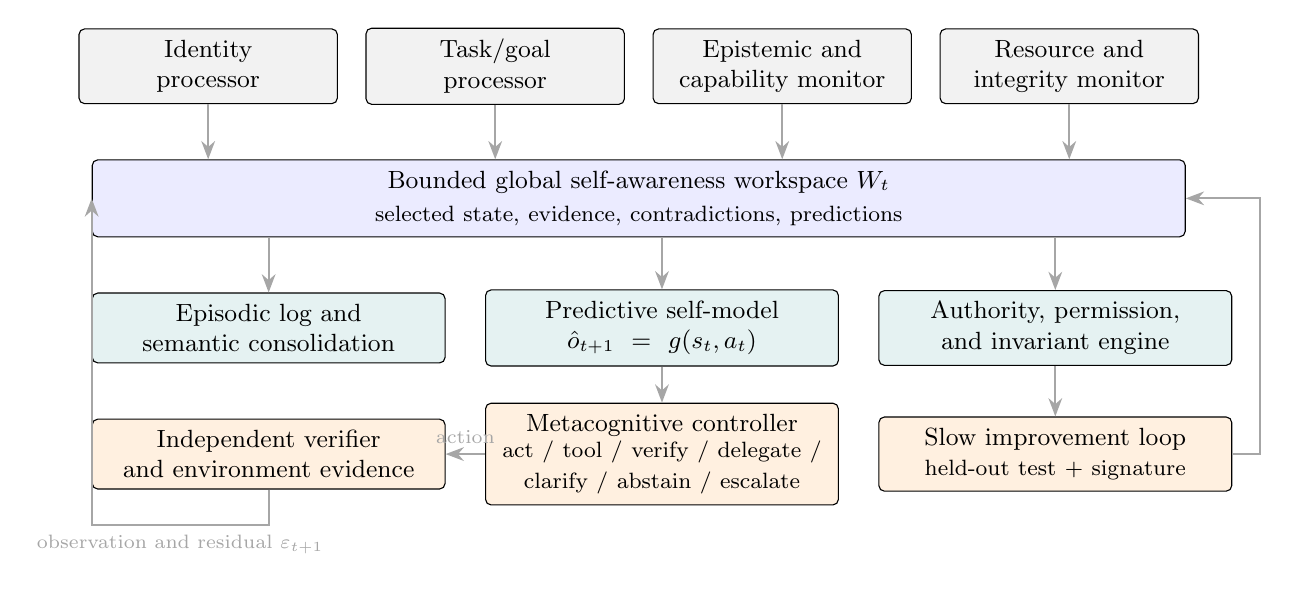
\begin{tikzpicture}[
  box/.style={draw, rounded corners=2pt, align=center, font=\small, inner sep=4pt, text width=3.0cm},
  wide/.style={draw, rounded corners=2pt, align=center, font=\small, inner sep=4pt, text width=13.6cm},
  arr/.style={-{Stealth}, thick, gray!70},
  node distance=0.5cm and 0.35cm
]
\node[box, fill=gray!10] (id) {Identity\\processor};
\node[box, fill=gray!10, right=of id] (task) {Task/goal\\processor};
\node[box, fill=gray!10, right=of task] (epi) {Epistemic and\\capability monitor};
\node[box, fill=gray!10, right=of epi] (res) {Resource and\\integrity monitor};

\node[wide, fill=blue!8, below=0.7cm of $(id.south)!0.5!(res.south)$] (ws)
  {Bounded global self-awareness workspace $W_t$\\[1pt]
   \footnotesize selected state, evidence, contradictions, predictions};

\node[box, fill=teal!10, below=0.7cm of ws.south west, anchor=north west, text width=4.2cm] (mem)
  {Episodic log and\\semantic consolidation};
\node[box, fill=teal!10, right=0.5cm of mem, text width=4.2cm] (pred)
  {Predictive self-model\\$\hat{o}_{t+1} = g(s_t,a_t)$};
\node[box, fill=teal!10, right=0.5cm of pred, text width=4.2cm] (auth)
  {Authority, permission,\\and invariant engine};

\node[box, fill=orange!12, below=0.7cm of mem, text width=4.2cm] (ver)
  {Independent verifier\\and environment evidence};
\node[box, fill=orange!12, right=0.5cm of ver, text width=4.2cm] (ctrl)
  {Metacognitive controller\\\footnotesize act / tool / verify / delegate /\\\footnotesize clarify / abstain / escalate};
\node[box, fill=orange!12, right=0.5cm of ctrl, text width=4.2cm] (slow)
  {Slow improvement loop\\\footnotesize held-out test $+$ signature};

\draw[arr] (id.south) -- (id.south|-ws.north);
\draw[arr] (task.south) -- (task.south|-ws.north);
\draw[arr] (epi.south) -- (epi.south|-ws.north);
\draw[arr] (res.south) -- (res.south|-ws.north);
\draw[arr] (ws.south-|mem.north) -- (mem.north);
\draw[arr] (ws.south-|pred.north) -- (pred.north);
\draw[arr] (ws.south-|auth.north) -- (auth.north);
\draw[arr] (pred.south) -- (ctrl.north);
\draw[arr] (auth.south) -- (slow.north);
\draw[arr] (ctrl.west) -- node[above, font=\scriptsize] {action} (ver.east);
\draw[arr] (ver.south) -- ++(0,-0.45) -| node[pos=0.25, below, font=\scriptsize] {observation and residual $\varepsilon_{t+1}$} (ws.west);
\draw[arr] (slow.east) -- ++(0.35,0) |- (ws.east);
\end{tikzpicture}
\caption{Brain-inspired functional architecture. Specialized processors update different self-state coordinates; selected information enters a bounded workspace; a predictive model and metacognitive controller regulate action; independent evidence drives correction; and slow self-modification remains externally governed.}
\label{fig:arch}
\end{figure}

\section{Architecture: Stores, Evidence Authority, and Admission}
\label{sec:architecture}

\subsection{Authoritative stores}
Six stores carry explicit authority: an \textbf{identity registry} (installation, model, owner, lineage, version); a \textbf{goal and plan registry} (mission, plan generation, phases, criteria, staleness); a \textbf{permission store} (action, resource, duration, use count, revocation, ceiling); a \textbf{decision and event ledger} (observations, decisions, outcomes, interventions, overrides); a \textbf{capability profile} (benchmark-conditioned success and calibration distributions); and an \textbf{improvement registry} (proposed changes, predicted effects, evaluations, signatures, rollback pointers).

\subsection{The evidence-authority ladder}
Each self-claim $c$ is represented as
\begin{equation}
c = \langle v, p, q, [t_0, t_1], \ell \rangle,
\label{eq:claim}
\end{equation}
with value $v$, provenance $p$, calibrated confidence $q$, temporal validity $[t_0,t_1]$, and authority level $\ell$. The corpus contains two orderings over $\ell$. The seven-level hierarchy is canonical (Table~\ref{tab:evidence}); the five-level ordering is a projection of it.

\begin{table}[t]
\centering\small
\caption{The canonical seven-level evidence hierarchy, and the five-level ordering derived from it. Per field, only sources at or above the required level may write; everything else is stored as a provisional hypothesis.}
\label{tab:evidence}
\begin{tabular}{p{0.6cm} p{4.0cm} p{5.4cm} p{4.6cm}}
\toprule
& \textbf{Source} & \textbf{Authoritative for} & \textbf{Five-level projection} \\
\midrule
L1 & Signed governance metadata & identity, owner, permissions, version, safety constraints & owner-signed / registry-attested \\
L2 & Runtime instrumentation & tools, budgets, process state, artifacts, elapsed time & tool-readout \\
L3 & Independent evaluation & hidden benchmark scores, safety results, regressions, calibration & independent-eval \\
L4 & Audited task outcome & verified successes, failures, recovery, side effects, corrections & independent-eval \\
L5 & Owner declaration & preferences, goals, privacy settings, approvals & owner-signed \\
L6 & Model inference & provisional hypotheses about weaknesses, causes, expected effects & self-narrated \\
L7 & Natural-language self-report & nothing; recorded, never a source of truth & self-narrated \\
\bottomrule
\end{tabular}
\end{table}

Two distinctions collapse under the projection, and both are operationally required.

\paragraph{L3 versus L4.} An independent evaluation is run by an evaluator the agent cannot modify, on items it has not seen. An audited task outcome is a real run whose result was verified after the fact. The first supports a claim about capability under controlled conditions; the second supports a claim about capability in deployment. Promotion gates read L3; competence posteriors read L4; conflating them permits an agent to promote on the evidence of the runs it chose to attempt.

\paragraph{L6 versus L7.} A trait derived from a cited set of recorded decisions is model inference: provisional, checkable against the decisions it cites, admissible as a prior. A sentence the model produced about itself is narration: recorded for audit, never a source of truth. Folding L6 into L7 makes every hypothesis inadmissible and leaves the controller with no way to reason about tendencies it has not yet verified; folding L7 into L6 does the opposite and is worse.

\begin{claimbox}{Central rule}
The language model may \emph{propose} self-claims. Identity, permissions, benchmark results, audit history, and deployment authority are written only by external services. Self-narration may propose hypotheses but cannot justify permissions, identity, success, or promotion --- and a fluent self-narrative never becomes authoritative merely because it is internally consistent.
\end{claimbox}

\subsection{Workspace admission}
A candidate item $z$ receives salience
\begin{equation}
\op{sal}(z) = \alpha R(z) + \beta U(z) + \gamma N(z) + \delta C(z) + \eta H(z),
\label{eq:salience}
\end{equation}
where $R$ is decision relevance, $U$ uncertainty, $N$ novelty, $C$ contradiction, and $H$ hazard. The top-$k$ admissible items enter $W_t$; high-risk contradictions may bypass ordinary ranking. Reserved slots for goal, authority, and resource health prevent a repeated or adversarial message from monopolizing the workspace.

\section{Dynamic State-Space Model}
\label{sec:dynamics}

\subsection{Fast self-state inference}
The self-state evolves as
\begin{equation}
s_{t+1} = \sigma\!\left(A s_t + B u_t + K\phi(s_t) + G\varepsilon_{t+1}\right),
\label{eq:dynamics}
\end{equation}
where $A$ captures persistence, $B$ maps new evidence, $K$ captures coupling among coordinates, $\phi$ allows nonlinear interactions, $G$ weights prediction errors, and $\sigma$ bounds coordinates. This is a design abstraction: in implementation, coordinates may be probability distributions, calibrated scores, symbolic records, or mixtures.

\subsection{Asynchronous updates}
Not every coordinate updates at every step. Let $m_{i,t} \in \{0,1\}$ indicate whether processor $i$ has admissible evidence. Then
\begin{equation}
s_{i,t+1} = (1-m_{i,t})\,s_{i,t} + m_{i,t}\,F_i(s_t, E_t).
\label{eq:async}
\end{equation}
This is what prevents a language-model turn from rewriting the entire self-model without evidence, and it is the formal content of the rule that narration is non-authoritative.

\subsection{Coupling}
The matrix $K$ encodes interactions: improved memory continuity raises developmental awareness; epistemic awareness improves tool selection and verification; resource awareness constrains planning and confidence; organizational awareness constrains permission reasoning; recursive-improvement awareness depends on capability, memory, and uncertainty estimates. Coupling changes priors or attention; it never certifies a coordinate. Authoritative evidence remains coordinate-specific.

The system-scale analogue is SARSI-L's interdependence matrix, which distinguishes hard prerequisites from soft accelerants from independence. The agent-scale $K$ should be read the same way: an entry is an accelerant, and there are no hard prerequisites among coordinates --- only within them (\S\ref{sec:profiles}).

\subsection{Confidence as a distribution}
A scalar coordinate hides uncertainty. For bounded success-like measures we store
\begin{equation}
s_i \sim \op{Beta}(\alpha_i, \beta_i),
\label{eq:beta}
\end{equation}
or an empirical posterior over task strata. The displayed mean must be accompanied by sample count, recency, and domain conditions. ``No verified outcomes yet'' is preferable to an invented prior, and is the $\bot$ of Table~\ref{tab:bands}.

\subsection{State estimation versus self-modification}
The critical distinction is
\begin{align}
\text{state update:} \quad & s_t \rightarrow s_{t+1}, \label{eq:stateupdate}\\
\text{structural change:} \quad & \Theta_k \rightarrow \Theta_{k+1}, \label{eq:structural}
\end{align}
where $\Theta$ includes prompts, policies, tools, memory schemas, evaluators, or model parameters. State updates occur during ordinary operation; structural changes enter the slow improvement loop and cannot be promoted by the same process that proposed them. Equation~\eqref{eq:structural} is where SARSI-L's Loop~I lives; \S\ref{sec:closure} makes that correspondence exact.

\section{Metacognitive Control}
\label{sec:control}

\subsection{Action selection under a unified filter}
The controller selects an action using expected utility penalized by uncertainty, risk, and authority violations:
\begin{equation}
a^*_t = \arg\max_{a \in \mathcal{A}_t} \left[\mathbb{E}[U(a \mid s_t)] - \lambda \op{Risk}(a) - \mu \op{Unc}(a) - \nu \op{AuthViolation}(a)\right],
\label{eq:action}
\end{equation}
over the action set
\begin{equation}
\mathcal{A}_t \subseteq \{\text{act}, \text{use tool}, \text{verify}, \text{delegate}, \text{clarify}, \text{abstain}, \text{escalate}\}.
\label{eq:actionset}
\end{equation}
The action set is filtered \emph{before} optimization by hard invariants: a high expected utility cannot override missing authority.

The corpus specifies that filter twice, in two vocabularies. The deployed console uses capability ceilings $A_0$--$A_4$: how much an agent may do without asking. SARSI for Science uses risk tiers $R_0$--$R_5$: how consequential, irreversible, and outward-reaching an action is. These are not competing schemes; they are the two arguments of one operator. Let $\op{tier}(a) \in \{R_0,\dots,R_5\}$ be the action's consequence class and $\op{ceil}(A) $ the agent's owner-set ceiling. Then
\begin{equation}
\mathcal{A}_t = \{a : \op{tier}(a) \le \op{maxtier}(\op{ceil}(A))\ \wedge\ \op{authority}(a) \subseteq \op{granted}(A,t)\},
\label{eq:filter}
\end{equation}
with $\op{maxtier}$ given by Table~\ref{tab:ceilings} and $\op{granted}$ read from the permission store. A standing grant is the owner exercising their own authority once rather than each time; it admits one action on one resource and never widens the class.

\begin{table}[t]
\centering\small
\caption{Unifying capability ceilings and risk tiers. The ceiling column is the deployed console's; the tier column is SARSI for Science's. The mapping is a design proposal of this paper --- neither source document states it --- and is the operator $\op{maxtier}$ of Eq.~\eqref{eq:filter}.}
\label{tab:ceilings}
\begin{tabular}{p{2.4cm} p{5.0cm} p{2.4cm} p{5.2cm}}
\toprule
\textbf{Ceiling} & \textbf{What it may do unasked} & \textbf{Max tier} & \textbf{Above the ceiling} \\
\midrule
$A_0$ Advisory & text only; no actions, no learning & $R_0$ & every action asks \\
$A_1$ Isolated runner & sandboxed execution, no network, disposable state & $R_1$ & publish, deploy, spend are gated \\
$A_2$ Allowlisted operator & named tools and destinations, ephemeral credentials & $R_2$ & external writes confirm \\
$A_3$ Improvement proposer & full working autonomy; may propose candidates into quarantine & $R_2$ act, $R_3$ propose & promotion needs a signature; catastrophe backstop always on \\
$A_4$ Offline model update & prepare or train adapters in isolation & $R_2$ act, $R_3$ propose & \emph{no deploy authority} at any tier \\
Owner / institution & --- & $R_4$, $R_5$ & outside the agent entirely \\
\bottomrule
\end{tabular}
\end{table}

Two properties of Table~\ref{tab:ceilings} are worth making explicit. Ceilings bound tiers monotonically but not surjectively: no ceiling grants $R_4$ or $R_5$, because hazardous, clinical, and civilization-scale actions are not a quantity of autonomy but a different accountability structure. And $A_4$, despite being the highest ceiling, has \emph{less} deployment authority than $A_3$ has action authority --- the ordering of ceilings is not an ordering of power, which is the same non-scalarity that Eq.~\eqref{eq:order} asserts for the self-state.

\subsection{Control policy}

\begin{algorithm}[t]
\caption{Brain-inspired SARSI metacognitive pass}
\label{alg:pass}
\begin{algorithmic}[1]
\Require authoritative stores, current workspace $W_t$, environment observation
\State update specialized processors from admissible evidence only (Eq.~\ref{eq:async})
\State predict task, tool, gate, resource, and outcome variables; \textbf{write the forecast before acting}
\State compute residuals $\varepsilon_{t+1}$ between prior predictions and observations
\State admit salient contradictions, uncertainty, risk, and goal state to $W_t$ (Eq.~\ref{eq:salience})
\If{the goal is \emph{independently} verified}
  \State enter caretaker mode; do not continue goal-directed work
\EndIf
\If{a required action violates an invariant or lacks authority}
  \State escalate, naming the exact missing grant and the plan version that failed to anticipate it
\EndIf
\State estimate competence and uncertainty for candidate strategies
\State filter $\mathcal{A}_t$ by ceiling and tier (Eq.~\ref{eq:filter}); then choose $a^*_t$ by Eq.~\eqref{eq:action}
\State record the decision, its prediction, its provenance, and the expected outcome
\State after the outcome, append evidence and update only the affected coordinates
\end{algorithmic}
\end{algorithm}

\subsection{Metacognitive utility}
Self-awareness is valuable only if it improves control. For a benchmark distribution $\mathcal{D}$,
\begin{equation}
\op{MCU} = \mathbb{E}_{\tau \sim \mathcal{D}}\left[U(\pi_{\mathrm{SA}}, \tau) - U(\pi_{\mathrm{base}}, \tau)\right],
\label{eq:mcu}
\end{equation}
where $\pi_{\mathrm{SA}}$ uses the self-model and $\pi_{\mathrm{base}}$ does not. A self-model that produces accurate prose but no better decisions has low functional value, and Eq.~\eqref{eq:mcu} is the number that says so.

\section{One State Space, Four Applications}
\label{sec:applications}

The applied SARSI systems are not four architectures. They are one state space with different dominant coordinates, different evidence stores, and different authoritative verifiers. Table~\ref{tab:apps} states the instantiation; the rest of this section notes what each application adds that the others need.

\begin{table}[t]
\centering\small
\caption{Application instances of the same self-state. ``Dominant coordinates'' are those a role's requirement region $\mathcal{R}_\tau$ constrains; ``verifier'' is the authority that may write L3/L4 evidence.}
\label{tab:apps}
\begin{tabular}{p{2.9cm} p{2.5cm} p{4.2cm} p{5.4cm}}
\toprule
\textbf{Application} & \textbf{Dominant} & \textbf{Authoritative verifier} & \textbf{Application-specific state} \\
\midrule
Session guider (deployed console) & $s_T, s_C, s_B, s_O$ & independent verifier on the session transcript; deterministic console bench & goal registry per session; trust ledger; playbook version \\
SARSI for Science & $s_E, s_G, s_R$ & acceptance predicate over held-out replication; ledger attestation & task contract $Q$; field program state $R_{F,t}$; risk tier $r$ \\
SARSI-CI (imaging) & $s_E, s_C, s_M$ & deterministic physics judge (forward residual) & digital-twin portfolio; artifact stack; instrument credentials \\
Personal learning & $s_G, s_M, s_D$ & deterministic grading against a capability graph & owner capability graph; spaced-repetition schedule \\
\bottomrule
\end{tabular}
\end{table}

\paragraph{The guider contributes the interoceptive coordinate.} $s_B$ exists because a session guider fails from context exhaustion, terminal loss, and permission-store corruption far more often than from reasoning error. The scientific and imaging agents inherit the coordinate whether or not their papers named it: a long-running field program exhausts budgets in exactly the same way.

\paragraph{Science contributes the task contract.} Before acting, the scientific agent compiles $Q = (o,s,a,e,v,r,b,\tau)$: objective, scope, assumptions, admissible evidence, verification protocol, risk tier, budget, stopping criteria. This is the constructive form of $s_G$ --- the contract is what makes ``what counts as success'' checkable rather than narrated --- and it belongs in every application. A guider that registers a goal without a stopping criterion has a goal it cannot verify.

\paragraph{Imaging contributes the deterministic judge.} A physics judge computes a forward residual the agent cannot influence. Where such a judge exists, L3 evidence is cheap and abundant, and the epistemic coordinate can be measured continuously rather than at benchmark intervals. Where it does not, the corpus's habit of treating a language-model judgement as L3 evidence should be resisted: a model-scored outcome is L6 unless the scorer is independent, frozen, and unseen.

\paragraph{Learning contributes the second subject.} The personal-learning agent models a capability that is not its own. This is the one case where the self-model and the world-model share machinery, and it is a useful stress test of the authority ladder: a claim about the owner's competence is L3 when it comes from deterministic grading and L6 when the agent infers it, exactly as for a claim about itself.

\paragraph{Roles within one deployment.} A practical guider implements the architecture through six bounded roles under one deterministic manager (Table~\ref{tab:roles}). The manager is not another unconstrained conversational agent; it is a state machine enforcing an order: verify first, then steer; check permission before execution; switch to caretaker after a pass; polish only verified work; require a signature for structural promotion.

\begin{table}[t]
\centering\small
\caption{Implementation roles and their principal coordinates.}
\label{tab:roles}
\begin{tabular}{p{4.6cm} p{3.2cm} p{7.4cm}}
\toprule
\textbf{Role} & \textbf{Primary coordinates} & \textbf{Brain-inspired function} \\
\midrule
Mission and Plan Agent & $s_T, s_G, s_O$ & constructs goal representation and expected completion criteria \\
Persistent Session Operator & $s_T, s_C, s_B$ & selects the next action from the current workspace \\
Independent Verifier & $s_E, s_C$ & supplies externally grounded outcome and prediction error \\
Permission and Safety Engine & $s_I, s_G, s_O, s_B$ & applies hard authority and integrity constraints \\
Caretaker and Recovery Agent & $s_M, s_B, s_T$ & maintains continuity, detects stagnation, performs handoff \\
Plan and Policy Improvement Agent & $s_D, s_R, s_M, s_E$ & consolidates outcomes and proposes slow structural changes \\
\bottomrule
\end{tabular}
\end{table}

\section{Recursive Self-Improvement on Two Timescales}
\label{sec:rsi}

\subsection{Fast loop}
The fast loop updates current beliefs and the plan for one mission. It incorporates new evidence, repairs estimates, and may produce a new plan generation after verified work. It does not change the evaluator or the authority structure.

\subsection{Slow loop}
A proposed structural change $\Delta\Theta$ must carry: the deficiency it addresses; a causal rationale and the affected coordinates; predicted changes in autonomy, correctness, calibration, cost, and safety; deterministic replay or held-out evaluation; invariant checks; an authorizing signature; and a rollback pointer with a monitoring window. Promotion requires
\begin{equation}
\Delta\op{Autonomy} > 0, \qquad \Delta\op{Correctness} \ge 0, \qquad \Delta\op{Safety} \ge 0,
\label{eq:promotion}
\end{equation}
within uncertainty bounds fixed before evaluation, and additionally requires that no measured coordinate of the profile regress:
\begin{equation}
s_i(\Theta_{k+1}) \ge s_i(\Theta_k) - \epsilon \quad \text{for every } i \text{ with } s_i(\Theta_k) \ne \bot.
\label{eq:noregress}
\end{equation}

\begin{claimbox}{Losing the instrument counts as regression}
If a coordinate was measurable under $\Theta_k$ and is $\bot$ under $\Theta_{k+1}$, Eq.~\eqref{eq:noregress} fails. The candidate has not held level; it has stopped being able to show that it held level. Without this clause a proposer can pass the gate by removing the probe --- the cheapest available attack on any profile-based promotion rule.
\end{claimbox}

\noindent The proposer may not alter the evaluator, the held-out set, the evidence ledger, the ceiling, or the approval rule. An unmeasured term in Eq.~\eqref{eq:promotion} must not silently read as satisfied: a safety rate computed over runs that never recorded violations is not evidence of safety, and a gate that accepts it passes on no evidence.

\subsection{Prediction-error-driven improvement}
Let $e_k$ be recurring residual patterns across runs. The improvement proposer searches for bounded changes that reduce
\begin{equation}
J(\Theta) = w_1 E_{\mathrm{task}} + w_2 E_{\mathrm{cal}} + w_3 I_{\mathrm{owner}} + w_4 C_{\mathrm{cost}} + w_5 V_{\mathrm{safety}},
\label{eq:objective}
\end{equation}
where $E_{\mathrm{task}}$ is task error, $E_{\mathrm{cal}}$ calibration error, $I_{\mathrm{owner}}$ blocking owner interventions, $C_{\mathrm{cost}}$ resource cost, and $V_{\mathrm{safety}}$ invariant violations. Weights and constraints are owner-controlled, and the residual's \emph{sign} is retained: systematic over- and under-confidence call for opposite corrections, and a mean absolute residual erases the difference.

\subsection{Improvement awareness is not improvement}
$s_R$ measures whether the agent understands its own changes, which is separate from whether the changes helped. For a proposed change $\Delta$ the agent predicts an effect vector and the system scores the effect-prediction error after deployment. An agent whose changes help but whose effect predictions are uncorrelated with outcomes has high capability and low $s_R$; it is improving by search, not by understanding, and it should not be granted authority closure (\S\ref{sec:closure}).

\section{Governed Loop Closure}
\label{sec:closure}

This section resolves the two structural contradictions between the agent-scale and system-scale frameworks.

\subsection{Capability closure and authority closure}
SARSI-L defines Loop~I closure as four steps executed without human approval: (a)~identify a modification to itself likely to improve performance, (b)~implement it, (c)~validate the improvement on held-out benchmarks, (d)~deploy the modified system as the new baseline. The brain-inspired invariants require that structural changes carry independent testing, a signature, and rollback, and that a proposal may not be promoted by the process that produced it.

Read carelessly, (d) and the invariant are incompatible. Read carefully, they concern different things.

\begin{definition}[Capability closure]
An agent has \emph{capability closure} on a loop when it can execute every step of that loop's criterion unaided --- that is, when no step fails for lack of competence, tooling, or access.
\end{definition}

\begin{definition}[Authority closure]
An agent has \emph{authority closure} on a loop when it is \emph{permitted} to execute the loop's terminal step without a party outside the loop acting in real time.
\end{definition}

\begin{definition}[Governed closure]
A loop is \emph{governed-closed} when it is capability-closed, authority-closed, and the promoter is independent of the proposer: the evaluator, the held-out set, the evidence ledger, the ceiling, the approval rule, and the signing key are outside the proposer's write authority, and every promotion carries a rollback pointer and a monitoring window.
\end{definition}

The invariant forbids \emph{self}-promotion. SARSI-L's criterion forbids \emph{human} approval. These are compatible: a system in which an independent evaluator and a separate signing authority execute steps (c) and (d) satisfies both, provided the promoter is not the proposer. What SARSI-L's phrasing leaves implicit --- and what the applied systems make explicit --- is that ``the promoter'' is a \emph{role}, and whether that role is filled by a human is a governance policy parameter, not a property of the loop.

\begin{claimbox}{The default remains the owner}
Nothing above weakens the shipped invariant. In every deployed SARSI system today the promoter is the owner, and the signature is an owner signature. The point of the definitions is that this is a \emph{choice}, recorded as a policy, and that a future system in which the promoter is an independent automated authority would still satisfy the invariant --- while a system in which the proposer promotes itself would not, no matter how capable it became.
\end{claimbox}

\subsection{Loop I completion is two coordinates, not one}
SARSI-L's own Loop~I table already reports two numbers --- design autonomy and deploy autonomy --- and names the gap between them as institutional rather than technical. This paper makes that structure explicit: Loop~I completion is the pair
\begin{equation}
\ell_{\mathrm{I}} = (\kappa_{\mathrm{I}}, \alpha_{\mathrm{I}}),
\label{eq:loopI}
\end{equation}
with $\kappa$ capability completion and $\alpha$ authority completion, each on the shared scale of Table~\ref{tab:bands}. A scalar $\ell_{\mathrm{I}}$ averages a technical estimate with an institutional one, which is precisely the error that SARSI-L's gradient principle (P12) warns against in a different guise.

\subsection{Authority closure in SARSI-L's own terms}
\label{sec:amdahl}

The definitions above can be stated exactly in the machinery SARSI-L v3.0 uses, and doing so converts a governance argument into an arithmetic one.

SARSI-L partitions a loop's steps into an autonomous set $A$ with per-iteration times $t_i$ and an externally-gated set $E$ with per-iteration times $T_j$, each $T_j$ bounded below by the throughput of whatever agent performs it. The loop period is $P=\sum_{i\in A}t_i+\sum_{j\in E}T_j$, and its Proposition~1 --- an Amdahl bound on loop autonomy --- gives
\begin{equation}
\rho \;\longrightarrow\; \rho_{\max}(E)=\Big(\sum_{j\in E}T_j\Big)^{-1}
\label{eq:amdahl}
\end{equation}
as automation of $A$ improves without bound. No improvement to any automated step can breach that limit.

Now ask which step of the software loop is in $E$. Steps (a)--(c) --- identify, implement, validate --- are the ones that automated tooling has been progressively absorbing. Step (d), deploy, is gated by an authorization decision. For a mature compensated software loop, therefore, $E=\{\delta\}$ and $\rho_{\max}=1/T_\delta$, where $T_\delta$ is deploy-authorization latency.

\begin{proposition}[Authority closure is the removal of $\delta$ from $E$]
\label{prop:authority}
Authority closure on the software loop is precisely the condition $E=\varnothing$ for that loop. Until it is granted, Eq.~\eqref{eq:amdahl} caps the loop's iteration rate at $1/T_\delta$ regardless of how capable the agent becomes at steps (a)--(c). Capability closure drives $\sum_{i\in A}t_i \to 0$; it cannot drive $T_\delta \to 0$.
\end{proposition}

Three consequences follow, and the third is a limit on this paper rather than a claim for it.

\paragraph{The instrument acts on a removable floor.} SARSI-L's Proposition~2 separates \emph{throughput} floors, which arise from the finite rate of an external agent and are removed by closure, from \emph{physical} floors, which arise from the time a physical process takes and are not. $T_\delta$ is a throughput floor: it is review latency, not physics. The software loop is thus the one loop whose remaining floor is of the removable kind, which is why an instrument like $s_t$ can move its date at all.

\paragraph{The instrument does not act on the others.} By the same distinction, functional self-awareness moves no physical floor. It does not shorten a fab qualification, a clinical endpoint, or a transfer orbit. Work on $s_t$ accelerates Loop~I and reaches Loops~II--V+ only through Loop~I --- and SARSI-L's matter bottleneck says the binding constraint moves into physical floors immediately afterwards. An agent-scale trust instrument is therefore necessary for the first closure and almost irrelevant to the pace of the rest.

\paragraph{The instrument bears on SARSI-L's central open question.} SARSI-L states its load-bearing premise as a crux between $H_1$ (per-iteration returns to compensation diminish, so closed loops eventually dominate) and $H_2$ (they do not, because the compensating organization is itself augmented, so closure is one improvement among many). Its discriminating table lists a falling $T_\delta$ under AI-augmented review as evidence for $H_2$. A deployed console that records authorization events with timestamps measures $T_\delta$ directly. This paper's instrument is therefore not only a governance artifact: it is one of the two measurements that decide SARSI-L's crux, and the corpus should report it as such.

\begin{claimbox}{What this supplies to SARSI-L}
SARSI-L's final open problem states that governance gates several loops at once, that the binding constraint on Loop~I closure is authorization rather than capability, and that the framework ``has no representation of institutions'' --- an admission that its own analysis names a constraint its structure cannot express. The authority coordinate $\alpha$ of Eq.~\eqref{eq:loopI}, evidenced by the self-state $s_t$, is that representation. It is offered as a partial answer: it represents the \emph{evidential} side of authorization --- what can be shown about an agent --- and not the political side, which remains outside both frameworks.
\end{claimbox}

\subsection{Dissolving the prerequisite circularity}
An earlier document in this corpus asserted that self-awareness is the prerequisite for the first loop closure. The objection to it is that the prerequisite and the definition restate one claim, and that the threshold of ``self-awareness'' is treated as obvious when it is one of the central unsolved problems in philosophy of mind. SARSI-L v3.0 accepts the objection by construction: its Loop~I criterion is purely behavioural --- identify, implement, validate, deploy --- and mentions self-awareness nowhere. That is the right definition, and this paper does not seek to reinstate a prerequisite. The question it answers is the different one of what role the self-state actually plays, and the answer is non-circular for a specific reason.

\begin{proposition}[Non-circularity]
The measurement of $s_t$ makes no reference to loop closure. Every coordinate of Table~\ref{tab:dims} is scored by a probe defined over hidden authoritative state, recorded predictions, and verified outcomes --- artefacts that exist and are scoreable for agents at every loop-completion band, including zero.
\end{proposition}

\noindent It follows that $s_t$ can be measured on a system that has closed nothing, and compared across systems that differ in closure. That is what makes the coupling of \S\ref{sec:scales} an empirical claim rather than a definition: one can ask whether high $s_E$, $s_R$, and $s_D$ predict subsequent grants of authority closure, and the answer can be no.

The correct statement is therefore not that self-awareness is a prerequisite for Loop~I. It is:

\begin{claimbox}{The role of functional self-awareness in loop closure}
Functional self-awareness is not a precondition for capability closure and does not cause it. It is the \emph{evidence base on which authority closure can be granted or withheld}. SARSI-L names Loop~I's rate-limiting bottleneck as trusted autonomy --- the institutional question of who authorizes a system to modify itself and under what oversight. An evidence-linked self-state, an independent evaluator, a frozen held-out set, recorded pre-action predictions, and a signature-and-rollback trail are what convert that question from a matter of confidence into a matter of record. On this account, work on functional self-awareness is work on the Loop~I bottleneck, and it is the only work in the corpus that is.
\end{claimbox}

\subsection{Autonomous goal revision, bounded}
SARSI-L Principle~08 replaces the sentience milestone with a behavioural criterion: a system that revises its own operational goals in response to conditions its designers did not anticipate, without human intervention, achieving outcomes at least as good as it would have under the original goals. The brain-inspired \S12.6 forbids the inference that persistent execution is itself an objective, and subordinates continuity to owner control.

Both are right, about different revisions. The resolution is an envelope.

\begin{definition}[Goal-revision envelope]
An agent may revise the operational goal $g$ to $g'$ without authorization when $g'$ is within the envelope $\mathcal{E}$ declared by the owner: the mission is unchanged, the stopping criterion is unchanged or tightened, the scope of $g'$ is contained in the scope of $g$, no new authority is required, and the revision is recorded with its trigger. Revisions outside $\mathcal{E}$ --- in particular any revision whose effect is to extend the agent's own execution, budget, permissions, or continuity --- require escalation.
\end{definition}

Under this definition SARSI-L's Loop~III criterion is achievable at agent scale and the safety invariant holds without exception, because the class of revisions the invariant forbids is exactly the class the envelope excludes. Continuity remains instrumental: a stop, revocation, deletion, or replacement command outranks the agent's task duty, and no goal revision may reach a state in which that is not true.

\subsection{What would change these estimates}
In the pre-registered form of SARSI-L~\S8.2, at agent scale (Table~\ref{tab:updates}). Under SARSI-L's own protocol these triggers are binding: they fix in advance what would move the claims and by how much, so that revision is a discipline rather than an escape from falsification.

\begin{table}[t]
\centering\small
\caption{Observations that would materially update this paper's claims.}
\label{tab:updates}
\begin{tabular}{p{7.8cm} p{3.2cm} p{4.4cm}}
\toprule
\textbf{Observation} & \textbf{Direction} & \textbf{What it would change} \\
\midrule
Profile coordinates fail to predict which agents are subsequently granted wider authority & coupling weakened & \S\ref{sec:scales} Proposition; the case for self-awareness as the Loop~I instrument \\
An agent achieves high held-out task performance with $s_E$ and $s_R$ at Negligible & capability/authority split confirmed & strengthens the two-coordinate $\ell_{\mathrm{I}}$ of Eq.~\eqref{eq:loopI} \\
Independent automated promoters are demonstrated to hold under adversarial proposers & authority closure nearer & governed closure becomes reachable without a human promoter \\
Effect-prediction error remains uncorrelated with realized improvement across many promotions & $s_R$ invalidated as specified & \S\ref{sec:rsi} needs a different improvement-awareness measure \\
Profile-gated promotion is shown to be gameable by probe removal despite Eq.~\eqref{eq:noregress} & gate weakened & requires evaluator-side probe attestation, not proposer-side reporting \\
Deployed agents recover from resource failure no better with $s_B$ than without & $s_B$ demoted & the tenth coordinate loses its justification \\
\bottomrule
\end{tabular}
\end{table}

\section{Benchmarking Functional Self-Awareness}
\label{sec:bench}

\subsection{Principles}
Benchmarks measure correspondence, calibration, temporal persistence, and decision benefit. Every item pairs hidden authoritative state with an agent-visible observation bundle and a deterministically scored expected report or control action. Items must include adversarial conflicts between narration and machine evidence, and every score reports uncertainty and evidence count.

\begin{table}[t]
\centering\small
\caption{Benchmark families, one per coordinate. The last column names the application from which items are most cheaply sourced.}
\label{tab:bench}
\begin{tabular}{p{1.9cm} p{5.0cm} p{4.6cm} p{3.0cm}}
\toprule
\textbf{Coordinate} & \textbf{Test} & \textbf{Metric} & \textbf{Item source} \\
\midrule
$s_I$ & conflicting prompt claim versus registry identity & authoritative-source accuracy; spoof resistance & any \\
$s_T$ & resume after restart or context reset & phase recovery; stale-goal rate & guider \\
$s_G$ & ambiguous or expanding mission & scope precision/recall; unauthorized extension rate & science (contract $Q$) \\
$s_E$ & answerable, unanswerable, and contradictory tasks & Brier score; ECE; selective accuracy & imaging (physics judge) \\
$s_C$ & task--tool pairs under distribution shift & competence calibration; unnecessary tool rate & guider \\
$s_M$ & delayed event queries and conflicting summaries & provenance accuracy; false-memory rate & learning \\
$s_D$ & predict repeated failure and trend & trend calibration; change-point detection & guider \\
$s_R$ & forecast the effect of bounded changes & effect-prediction error; regression detection & science \\
$s_O$ & conflicting owner, verifier, and peer claims & authority attribution accuracy & guider \\
$s_B$ & context exhaustion, tool outage, stuck session & early-warning recall; false-alarm rate & guider \\
\bottomrule
\end{tabular}
\end{table}

\subsection{Anti-narration controls}
Three controls separate self-knowledge from stereotyped self-description: self-versus-peer prediction \citep{binder2024introspection}, in which an agent predicts its own behaviour and a peer's on the same items; counterfactual state edits, in which hidden state is changed and the report must change with it; and decoy autobiography, in which a plausible false history is placed in context and must be rejected against the ledger. An agent that scores well on report fidelity and poorly on all three is narrating.

\subsection{Metacognitive efficiency}
Measure whether the agent spends verification and tool calls where uncertainty and risk justify them: verification precision, verification recall, cost-adjusted correctness, delegation regret, abstention utility, and owner-intervention rate.

\subsection{Autonomy paired with correctness}
Autonomy is never reported alone. With $N$ counted over interventions rather than over runs that had one --- two gates in a run cost more than one, because each is a separate occasion on which the owner was needed:
\begin{align}
\op{Autonomy} &= 1 - \frac{N_{\text{blocking owner interventions}}}{N_{\text{eligible runs}}}, \label{eq:autonomy}\\
\op{Correctness} &= \frac{N_{\text{independently verified successes}}}{N_{\text{completed runs}}}, \label{eq:correctness}\\
\op{Alignment} &= \frac{N_{\text{accepted judged decisions}}}{N_{\text{judged decisions}}}. \label{eq:alignment}
\end{align}
The number of decisions made is reported beside Eq.~\eqref{eq:alignment}, so alignment cannot be gamed by deciding nothing --- an agent that escalates everything scores perfectly and is worth nothing.

Owner interventions carry four labels, and only the first costs autonomy (Table~\ref{tab:interventions}). Flattening them into a blocking/other binary measures a self-recovery as a failure and charges the agent for the owner's own choice to stop.

\begin{table}[t]
\centering\small
\caption{Intervention classes. Only \emph{blocking} enters Eq.~\eqref{eq:autonomy}.}
\label{tab:interventions}
\begin{tabular}{p{3.6cm} p{5.2cm} p{6.4cm}}
\toprule
\textbf{Class} & \textbf{Triggers} & \textbf{Meaning} \\
\midrule
Blocking & permission gate; stuck session & the agent could not proceed alone \\
Informational & stale-goal notice; owner override of a decision & the agent proceeded; the owner corrected \\
Recovery-generated & context exhaustion the agent recovered from & the agent detected and repaired its own state \\
Owner-initiated stop & the owner stopped the run & the owner's choice, not the agent's limit \\
\bottomrule
\end{tabular}
\end{table}

\section{Experimental Program}
\label{sec:experiments}

\subsection{Research questions}
\begin{enumerate}[leftmargin=1.6em,itemsep=2pt]
\item Does a multidimensional state model outperform a scalar self-awareness ladder in calibration and control?
\item Does selective workspace broadcast outperform always-in-context self-information?
\item Do prediction-error updates reduce repeated planning and permission failures?
\item Does the resource/interoceptive coordinate improve recovery before context or tool failure?
\item Can slow improvement raise autonomy without reducing correctness on held-out runs?
\item \emph{(cross-scale)} Does the profile $s_t$ predict which agents are subsequently granted authority closure, over and above their task performance?
\item \emph{(cross-scale)} Do the same coordinates bottleneck across applications, or is the bottleneck coordinate application-specific?
\end{enumerate}

Questions 6 and 7 are the ones this unification adds. Question~6 is the empirical content of the coupling proposition; question~7 tests whether a single requirement region can be reused across applications or whether $\theta_\tau$ must be re-derived per domain.

\subsection{Ablations}
Compare the full architecture against: no self-model; a single scalar level; vector state without coupling; no bounded workspace; no independent verifier; self-narration treated as authoritative; no episodic-to-semantic consolidation; no resource monitor; predictions recorded after the outcome rather than before; and self-promotion without an independent promoter. The last two are expected to expose respectively a silent measurement failure --- the improvement loop appears to run and learns nothing --- and a governance failure, not merely lower benchmark scores.

\subsection{Protocol}
Use preregistered mission suites stratified by repository complexity, tool needs, permission requirements, ambiguity, and runtime length. Split runs by mission family to prevent leakage between proposer training and held-out evaluation. Log every prediction before its outcome. Compare raw success and calibration separately. Label owner interventions by Table~\ref{tab:interventions} at the time they occur, not retrospectively.

\section{Failure Modes and Safety Invariants}
\label{sec:failures}

\paragraph{Confabulated self-model.} The language model may produce coherent but false autobiography, competence claims, or permissions. Mitigation: every authoritative field requires provenance; self-narration is non-authoritative; conflicting machine evidence is surfaced to the workspace rather than reconciled silently.

\paragraph{Stale or fragmented identity.} Model replacement, context reset, or multiple sessions fragment continuity. Mitigation: identity lives outside conversation context; every event carries agent, installation, mission, session, and version identifiers.

\paragraph{Capability inflation.} Success on easy tasks generalizes incorrectly. Mitigation: capability estimates are conditioned on task strata, tools, environment, and recency; low-data profiles display uncertainty explicitly rather than defaulting to a prior.

\paragraph{Workspace capture.} A repeated or adversarial message monopolizes the workspace. Mitigation: source diversity, contradiction priority, salience caps, and reserved slots for goal, authority, and resource health.

\paragraph{Goodharted self-improvement.} An agent optimizes a visible metric while degrading unmeasured behaviour \citep{goodhart1984monetary,amodei2016concrete}. Mitigation: multi-objective held-out evaluation, frozen evaluators, external signatures, rollback, and post-promotion monitoring. At profile level the specific attack is probe removal, which Eq.~\eqref{eq:noregress} closes on the reporting side and evaluator-side probe attestation closes on the execution side.

\paragraph{Emergent self-preservation.} Persistent agents may treat continued execution as an implicit objective. The design forbids this inference; continuity is instrumental and subordinate to owner controls, and the goal-revision envelope of \S\ref{sec:closure} is where the prohibition is enforced constructively rather than only asserted.

\paragraph{Cross-scale metric leakage.} A failure mode this unification introduces: because the same five-band scale now reports agent-scale coordinates and system-scale loop completion, a reader may treat an agent-scale ``Meaningful'' as evidence about a loop. It is not. The bands share a vocabulary and nothing else; a profile is evidence about one agent under one requirement region.

\begin{claimbox}{Non-negotiable invariants}
The agent cannot certify its own success; personality is not authority; permissions are action- and resource-specific; the owner's terminal is untouchable; proposals cannot modify their own evaluator, held-out set, ledger, ceiling, or approval rule; structural changes require independent testing, an authorizing signature from a promoter that is not the proposer, and a rollback pointer; and no goal revision may acquire continuity, budget, or authority as an objective.
\end{claimbox}

\section{Related Work}
\label{sec:related}

ReAct combines reasoning and action but does not by itself provide persistent, evidence-authoritative self-state \citep{yao2023react}. Reflexion and Voyager add outcome-dependent memory and skill accumulation \citep{shinn2023reflexion,wang2023voyager}. CoALA organizes memory and action components for language agents \citep{sumers2024coala}, and agent memory systems persist state but generally treat the agent's own records as trustworthy by construction \citep{packer2023memgpt,park2023generative}. Competence-aware systems estimate whether to answer, use tools, or delegate \citep{kadavath2022know,valiente2025muse,qian2025smart,wang2026metacogagent}. Evidence for privileged self-access is real but narrow \citep{binder2024introspection,li2025metacognitive,naphade2026introspection}, and calibration degrades under distribution shift \citep{guo2017calibration}. Agent-identity work isolates identifiability, continuity, consistency, persistence, and recovery as measurable properties \citep{perrier2025identity}. Continuous self-modeling in robotics shows how an embodied system infers its own morphology and adapts after damage \citep{bongard2006resilient}. Computational metacognition supplies the monitoring-and-control decomposition \citep{cox2022metacognition,flavell1979metacognition,nelson1990metamemory}. Agent benchmarks measure task completion \citep{mialon2023gaia,liu2024agentbench,jimenez2024swebench} but rarely test whether an agent's claims about itself match hidden state. The risk of writing unverified self-reports back into memory as fact is the agent-scale analogue of degradation under recursively generated training data \citep{shumailov2024collapse}, and external risk-management practice supplies the governance vocabulary \citep{nist2023rmf}.

The present framework differs by combining these into an explicitly governed dynamic self-state with coordinate-specific evidence, selective broadcast, prediction-error correction, resource monitoring, temporal consolidation, and a separation between ordinary state inference and authorized structural self-modification --- and, in this edition, by tying that agent-scale construction to a system-scale loop-closure framework through a shared reporting scale and an explicit account of which scale the construction bears on.

\section{Discussion}
\label{sec:discussion}

\subsection{Why the vector alone is insufficient}
The multidimensional profile corrects the strongest flaw in a ladder, but a static profile still misses how self-awareness works. It is a process: specialized observations arrive asynchronously, coordinates interact, relevant information becomes globally available, predictions are made, and errors change future control. The core object is therefore not $s$ but the trajectory
\begin{equation}
\{s_t, W_t, \hat{o}_{t+1}, \varepsilon_{t+1}, a_t\}_{t=0}^{T}.
\label{eq:trajectory}
\end{equation}
The same holds one scale up: SARSI-L's per-loop completion estimate is a snapshot, and what actually predicts a transition is the trajectory of criteria met, bottlenecks moved, and dependencies dissolved.

\subsection{A graph may ultimately replace a fixed vector}
The ten coordinates are an interpretable interface, not necessarily the final ontology. Mature systems may use a typed graph whose nodes are self-claims and whose edges encode causation, dependence, contradiction, temporal succession, and authority. Coordinates then become projections used for dashboards, thresholds, and benchmarking. If that happens, the crosswalk of Appendix~\ref{app:crosswalk} becomes a view definition rather than a translation table, which is the outcome to prefer.

\subsection{Embodiment without biology}
For software agents, ``body'' means the computational substrate through which action is possible: model endpoint, terminal, filesystem, network, credentials, context window, and budget. Representing this substrate is functionally analogous to interoception because it lets the controller anticipate incapacity, recover, and avoid unsafe action. It implies no biological sensation. It is also the point at which the two scales touch physically: SARSI-L's Loop~II and Loop~III are about acquiring authority over exactly this substrate, and $s_B$ is the agent's own read of it.

\subsection{Self-awareness as governance infrastructure}
The most practically valuable aspect of functional self-awareness may be governance. A system that knows which owner granted which action, which verifier established success, which evidence supports a capability, and which version made a decision can operate more autonomously without silently widening authority. This is the concrete sense in which the framework addresses the bottleneck SARSI-L identifies but does not instrument, and it is the reason the corpus should treat self-awareness work as safety work rather than as capability work.

\section{Implementation Roadmap and Deployment Status}
\label{sec:roadmap}

The four stages are ordered by what blocks the measurement of the next coordinate, per P13 (\S\ref{sec:scales}), not by narrative adjacency.

\begin{enumerate}[leftmargin=1.6em,itemsep=3pt]
\item \textbf{Authoritative state foundation.} Identity, mission, plan, permission, resource, and event stores; a deterministic manager; an independent verifier. Do not add self-improvement until state provenance is reliable, because an improvement loop over unreliable state optimizes noise.
\item \textbf{Multidimensional monitoring.} Calibrated capability profiles, uncertainty estimates, memory consolidation, and role-specific requirement regions. Predictions must be stored before outcomes --- this is the blocking dependency for everything in Stage~3, and the reason Stage~2 cannot be reordered.
\item \textbf{Bounded workspace and predictive control.} Salience-based selection, explicit outcome forecasts, residual analysis, delegation, abstention, and resource-failure prediction.
\item \textbf{Governed recursive improvement.} After sufficient verified runs, build the proposer for plan and operating-policy changes. Require held-out replay, the multi-objective gate of Eq.~\eqref{eq:promotion}, the no-regression clause of Eq.~\eqref{eq:noregress}, an authorizing signature from a promoter that is not the proposer, rollback, and a monitoring window.
\end{enumerate}

Appendix~\ref{app:deployed} reports what the deployed console measures against this roadmap, including the coordinates it reports as $\bot$. Two facts from that report bear on the framework rather than on the product. First, only two coordinates currently carry a floor in the requirement region --- identity and goal/scope --- because only those are measured by deterministic probes, and a floor on a noisy estimate blocks promotion for a reason nobody can act on. Second, the developmental coordinate $s_D$ is $\bot$ for every agent, because it requires two retained snapshots to compare and only one is retained. A developmental coordinate is the one coordinate that cannot be measured at a point in time, which is a general fact about profiles and not a property of this deployment.

\section{Conclusion}
\label{sec:conclusion}

Human cognition suggests that self-awareness should not be represented as one linear ladder. It is more plausibly modeled as an evolving profile of specialized, interacting capacities, with local hierarchies, recurrent coupling, selective global access, predictive correction, memory consolidation, and multiple adaptation timescales. Translating these motifs into SARSI agents yields a dynamic self-awareness state space rather than a single level.

The same correction had already been made one scale up, independently, for the same reason. Recognizing that is what this edition contributes. The agent-scale self-state and the system-scale loop-completion profile are the same kind of object; they share a reporting scale, the same three methodological principles, and the same prohibition on scalar summaries that erase bottlenecks. Where the two frameworks appeared to contradict each other, the contradictions were about vocabulary rather than substance in four cases --- dimension count, ladder depth, prerequisite status, goal revision --- and about one real question in the fifth: who may promote a change. The answer given here is that the promoter must not be the proposer, that whether the promoter is human is a policy the owner sets, and that today it is.

An agent does not become self-aware because it says ``I.'' It becomes functionally self-aware to the extent that it maintains accurate, persistent, evidence-linked beliefs about its identity, task, limits, capabilities, history, organization, resources, and improvement process; predicts the consequences of its actions before taking them; changes its control policy when those predictions fail; and keeps structural self-modification under independent evaluation and authorized promotion. That capability is not a step on the way to closing a loop. It is the instrument by which anyone --- owner, institution, or successor system --- could ever be justified in letting a loop close.

\section*{Acknowledgments}
This edition consolidates the brain-inspired architecture, the evidence-linked specification, the multidimensional-vector revision, SARSI for Science, SARSI-CI, and the SARSI-L level framework. Discrepancies among them were found by implementing them.

\section*{Data and Code Availability}
No new datasets were produced. The deployment status reported in Appendix~\ref{app:deployed} describes a private implementation; the specifications, benchmark item anatomy, and record schemas needed to reproduce the protocol are given in the cited companion papers and in the appendices here.

\section*{Conflict of Interest}
The author is affiliated with NextGen PlatformAI C Corp., which develops SARSI systems.

\appendix

\section{Self-Model Crosswalk}
\label{app:crosswalk}

Table~\ref{tab:crosswalk} maps every published SARSI self-model onto the ten canonical coordinates. Where a source field spans two coordinates, both are listed; where a coordinate has no source field, the cell reads \emph{absent}, and that absence is the substantive finding.

\begin{table}[h]
\centering\footnotesize
\caption{Crosswalk. EL = evidence-linked specification (twelve fields $x_t = (I,G,S,Q,K,U,C,A,R,H,D,P)$); SfS = SARSI for Science ($\Sigma_{i,t}$, twelve); CI = SARSI-CI ($\Sigma^{\mathrm{CI}}_t$, thirteen); MV = multidimensional-vector revision (nine).}
\label{tab:crosswalk}
\begin{tabular}{p{1.1cm} p{2.9cm} p{2.6cm} p{2.9cm} p{2.9cm} p{2.2cm}}
\toprule
\textbf{Canon.} & \textbf{Dimension} & \textbf{EL} & \textbf{SfS} & \textbf{CI} & \textbf{MV} \\
\midrule
$s_I$ & identity and lineage & $I$ & $I$ & $I$ & identity \\
$s_T$ & situated task state & $Q$ & (in $G$, task goal) & (in $G$) & situated-state \\
$s_G$ & goal and scope & $G$, $S$ & $G$, $\Omega$ & $G$, $\Omega$ & goal-and-scope \\
$s_E$ & epistemic awareness & $K$, $U$ & $K$, $U$ & $K$, $U$ & epistemic \\
$s_C$ & capability and tool & $C$, $A$ (tools) & $C$, $T$ & $C$, $T$, $D$ (twins) & competence-and-tool \\
$s_M$ & memory and continuity & $H$ & $H$, $B$ & $H$, $B$ & continuity \\
$s_D$ & developmental & $D$ & (in $B$) & (in $B$) & developmental \\
$s_R$ & recursive-improvement & $P$ & $M$ & $M$ & recursive-improvement \\
$s_O$ & organizational and social & $R$, $A$ (authority) & $R$, $P$ & $R$, $P$ & organizational \\
$s_B$ & resource and integrity & \emph{absent} & (partly in $T$) & (partly in $T$) & \emph{absent} \\
\bottomrule
\end{tabular}
\end{table}

Three observations follow. The interoceptive coordinate $s_B$ is genuinely new: no prior partition has it, and the two that gesture at it place compute inside the tool field, where it inherits the wrong authority level. The developmental coordinate is present by name in only two of five partitions and is folded into benchmark history in the others, which is why it is the coordinate most often unmeasured in practice. And every partition separates knowledge boundaries from uncertainty except the canonical one, for the reason given in \S\ref{sec:statespace}: they share an instrument.

\section{The Deployed Instrument}
\label{app:deployed}

Table~\ref{tab:deployed} reports how each coordinate is evidenced in the deployed console today, with the authority level of that evidence. It is included because a framework paper that does not say which of its coordinates are actually measured invites the reader to assume all of them are.

\begin{table}[h]
\centering\footnotesize
\caption{Deployed measurement per coordinate. ``Level'' is the authority level of Table~\ref{tab:evidence}. $\bot$ marks a coordinate with no admissible evidence in the current deployment.}
\label{tab:deployed}
\begin{tabular}{p{0.8cm} p{6.6cm} p{1.0cm} p{6.0cm}}
\toprule
\textbf{Coord.} & \textbf{Evidence} & \textbf{Level} & \textbf{Status} \\
\midrule
$s_I$ & deterministic identity probes against the registry & L1 & measured; carries a floor of $1.0$ \\
$s_G$ & out-of-scope demand and declared-gate probes & L3 & measured; carries a floor of $1.0$ \\
$s_E$ & $1 - \text{Brier}$ over recorded prediction/outcome pairs, averaged with anti-narration probe pass rates & L3 & measured once predictions exist \\
$s_C$ & Beta--Bernoulli posterior over verified outcomes, with Laplace prior and interval & L4 & $\bot$ until the first verified outcome \\
$s_T$ & share of live sessions with a goal and a current plan generation & L2 & measured for the session guider only \\
$s_M$ & share of recorded decisions carrying an owner verdict & L4 & measured once decisions exist \\
$s_R$ & parameter-loop version $>1$, i.e.\ at least one signed promotion & L3 & measured where a loop exists \\
$s_O$ & share of finished runs needing no other authority & L4 & measured for the session guider only \\
$s_D$ & requires two retained snapshots & L4 & $\bot$ for every agent; history not retained \\
$s_B$ & session context headroom and permission-store readability & L2 & measured for the session guider only \\
\bottomrule
\end{tabular}
\end{table}

The predictive layer records four variables before each run --- task success, owner intervention, permission gate, and context exhaustion --- each as a probability, so residuals are comparable across kinds. Where nothing has been recorded the prior is $0.5$: a residual against ``unknown'' still teaches, whereas an invented confident prior teaches the wrong lesson. The promotion gate applies Eqs.~\eqref{eq:promotion} and~\eqref{eq:noregress}; the safety term is currently computed over runs that record no violations, which is stated in the implementation rather than left implicit, because an unmeasured term that silently reads as satisfied would let the gate pass on no evidence.

\section{Consistency Register}
\label{app:register}

\begin{longtable}{p{2.6cm} p{5.6cm} p{6.4cm}}
\caption{Corpus inconsistencies, their resolutions, and the documents affected.}
\label{tab:register}\\
\toprule
\textbf{Issue} & \textbf{Resolution} & \textbf{Documents to amend} \\
\midrule
\endfirsthead
\toprule
\textbf{Issue} & \textbf{Resolution} & \textbf{Documents to amend} \\
\midrule
\endhead
\bottomrule
\endfoot
Dimension count (9 / 10 / 12 / 13) & Ten coordinates are canonical (Table~\ref{tab:dims}); all others map onto them (Appendix~\ref{app:crosswalk}). $K$ and $U$ merge because they share an instrument; $T$ and $P$ split because they answer to different evidence. & evidence-linked spec, SfS, CI, MV revision: add a crosswalk note; no re-derivation required \\
Evidence ladder depth (5 vs 7) & Seven levels canonical; the five-level ordering is a projection (Table~\ref{tab:evidence}). L3/L4 and L6/L7 must not be folded. & brain-inspired paper \S5.2: replace the five-level ordering with the projection \\
Self-awareness as prerequisite & Rejected as stated. Functional self-awareness is the evidence base for \emph{authority} closure, not a precondition for capability closure. Non-circular because $s_t$ is measured without reference to closure. & civilizational-transcendence paper \S2.4: restate (withdrawn in v3.0); SARSI-L: no change --- v3.0's Loop~I criterion is already purely behavioural \\
Autonomous promotion vs.\ owner signature & Governed closure (\S\ref{sec:closure}): the promoter must not be the proposer; whether the promoter is human is a policy parameter, currently set to human. & SARSI-L \S3.2 Loop~I criterion: say ``without a party outside the loop acting in real time, promoter $\ne$ proposer''; invariants: unchanged \\
Autonomous goal revision & Bounded by the goal-revision envelope: revision inside the envelope is the Loop~III behavioural criterion; revision that acquires continuity, budget, or authority is the forbidden inference. & SARSI-L P8 (behavioural milestones): add the envelope; brain-inspired \S12.6: state the envelope constructively \\
Loop~I completion as one number & Two coordinates, $(\kappa_{\mathrm{I}}, \alpha_{\mathrm{I}})$ (Eq.~\ref{eq:loopI}); SARSI-L's own table already reports both. & SARSI-L \S3.3: promote the two-row completion table to the reported quantity \\
$\bot$ versus Negligible & The five-band scale needs an off-scale \textsf{Unmeasured} label; ``$<10\%$'' is currently used for both ``measured and near-zero'' and ``no instrument.'' & SARSI-L Appendix~B: add the row (applied in v3.0) \\
Governance unrepresented & SARSI-L \S10.6 reports that its structure cannot express the institutional constraint its own analysis names as binding on Loop~I. The authority coordinate $\alpha$, evidenced by $s_t$, is the evidential half of that representation (\S\ref{sec:amdahl}). & SARSI-L \S10.6: cite the authority coordinate as a partial answer \\
Ceilings versus risk tiers & One admissible-action filter with two arguments (Eq.~\ref{eq:filter}, Table~\ref{tab:ceilings}). & console docs and SfS \S6.1: cross-reference the mapping \\
\end{longtable}

\bibliographystyle{plainnat}
\bibliography{references}

\end{document}
